\documentclass[tikz,border=2pt]{standalone}
\usepackage{amsmath,amssymb}
\usepackage{tikz}
\usetikzlibrary{arrows.meta}

\begin{document}
% Anatomy of an optimization model: decision variables, objective function, functional
% constraints with their parameters, and domain (sign) restrictions.
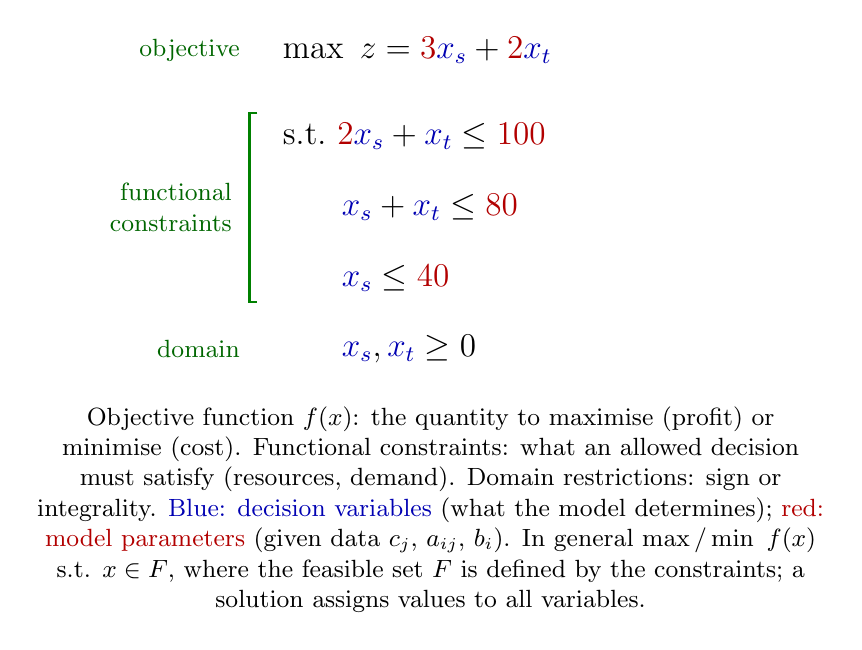
\begin{tikzpicture}[every node/.style={font=\small}, >={Latex[length=1.8mm]}]
	\node[anchor=west, font=\large] at (0,2.4) {$\max\ z=\textcolor{red!70!black}{3}\textcolor{blue!70!black}{x_s}+\textcolor{red!70!black}{2}\textcolor{blue!70!black}{x_t}$};
	\node[anchor=west, font=\large] at (0,1.3) {s.t.\ $\textcolor{red!70!black}{2}\textcolor{blue!70!black}{x_s}+\textcolor{blue!70!black}{x_t}\le\textcolor{red!70!black}{100}$};
	\node[anchor=west, font=\large] at (0.75,0.4) {$\textcolor{blue!70!black}{x_s}+\textcolor{blue!70!black}{x_t}\le\textcolor{red!70!black}{80}$};
	\node[anchor=west, font=\large] at (0.75,-0.5) {$\textcolor{blue!70!black}{x_s}\le\textcolor{red!70!black}{40}$};
	\node[anchor=west, font=\large] at (0.75,-1.4) {$\textcolor{blue!70!black}{x_s},\textcolor{blue!70!black}{x_t}\ge0$};
	\node[green!40!black, anchor=east] at (-0.3,2.4) {objective};
	\draw[green!50!black, thick] (-0.2,1.6) -- (-0.3,1.6) -- (-0.3,-0.8) -- (-0.2,-0.8);
	\node[green!40!black, anchor=east, align=right] at (-0.4,0.4) {functional\\ constraints};
	\node[green!40!black, anchor=east] at (-0.3,-1.4) {domain};
	\node[anchor=north, align=flush center, text width=10cm] at (2.0,-2.0) {Objective function $f(x)$: the quantity to maximise (profit) or minimise (cost). Functional constraints: what an allowed decision must satisfy (resources, demand). Domain restrictions: sign or integrality. \textcolor{blue!70!black}{Blue: decision variables} (what the model determines); \textcolor{red!70!black}{red: model parameters} (given data $c_j$, $a_{ij}$, $b_i$). In general $\max/\min\ f(x)$ s.t. $x\in F$, where the feasible set $F$ is defined by the constraints; a solution assigns values to all variables.};
\end{tikzpicture}
\end{document}
